\documentclass[11pt,a4paper]{report}
\usepackage[textwidth=37em,vmargin=30mm]{geometry}
\usepackage{calc,xunicode,amsmath,amssymb,paralist,enumitem,tabu,booktabs,datetime2,xeCJK,xeCJKfntef,listings}
\usepackage{tocloft,fancyhdr,tcolorbox,xcolor,graphicx,eso-pic,xltxtra,xelatexemoji}

\newcommand{\envyear}[0]{2025}
\newcommand{\envdatestr}[0]{2025-02-02}
\newcommand{\envfinaldir}[0]{webdb/2025/20250202/final}

\usepackage[hidelinks]{hyperref}
\hypersetup{
    colorlinks=false,
    pdfpagemode=FullScreen,
    pdftitle={Web Digest - \envdatestr}
}

\setlength{\cftbeforechapskip}{10pt}
\renewcommand{\cftchapfont}{\rmfamily\bfseries\large\raggedright}
\setlength{\cftbeforesecskip}{2pt}
\renewcommand{\cftsecfont}{\sffamily\small\raggedright}

\setdefaultleftmargin{2em}{2em}{1em}{1em}{1em}{1em}

\usepackage{xeCJK,xeCJKfntef}
\xeCJKsetup{PunctStyle=plain,RubberPunctSkip=false,CJKglue=\strut\hskip 0pt plus 0.1em minus 0.05em,CJKecglue=\strut\hskip 0.22em plus 0.2em}
\XeTeXlinebreaklocale "zh"
\XeTeXlinebreakskip = 0pt


\setmainfont{Brygada 1918}
\setromanfont{Brygada 1918}
\setsansfont{IBM Plex Sans}
\setmonofont{JetBrains Mono NL}
\setCJKmainfont{Noto Serif CJK SC}
\setCJKromanfont{Noto Serif CJK SC}
\setCJKsansfont{Noto Sans CJK SC}
\setCJKmonofont{Noto Sans CJK SC}

\setlength{\parindent}{0pt}
\setlength{\parskip}{8pt}
\linespread{1.15}

\lstset{
	basicstyle=\ttfamily\footnotesize,
	numbersep=5pt,
	backgroundcolor=\color{black!5},
	showspaces=false,
	showstringspaces=false,
	showtabs=false,
	tabsize=2,
	captionpos=b,
	breaklines=true,
	breakatwhitespace=true,
	breakautoindent=true,
	linewidth=\textwidth
}






\newcommand{\coverpic}[2]{
    % argv: itemurl, authorname
    Cover photo by #2~~(\href{#1}{#1})
}
\newcommand{\makeheader}[0]{
    \begin{titlepage}
        % \newgeometry{hmargin=15mm,tmargin=21mm,bmargin=12mm}
        \begin{center}
            
            \rmfamily\scshape
            \fontspec{BaskervilleF}
            \fontspec{Old Standard}
            \fontsize{59pt}{70pt}\selectfont
            WEB\hfill DIGEST
            
            \vfill
            % \vskip 30pt
            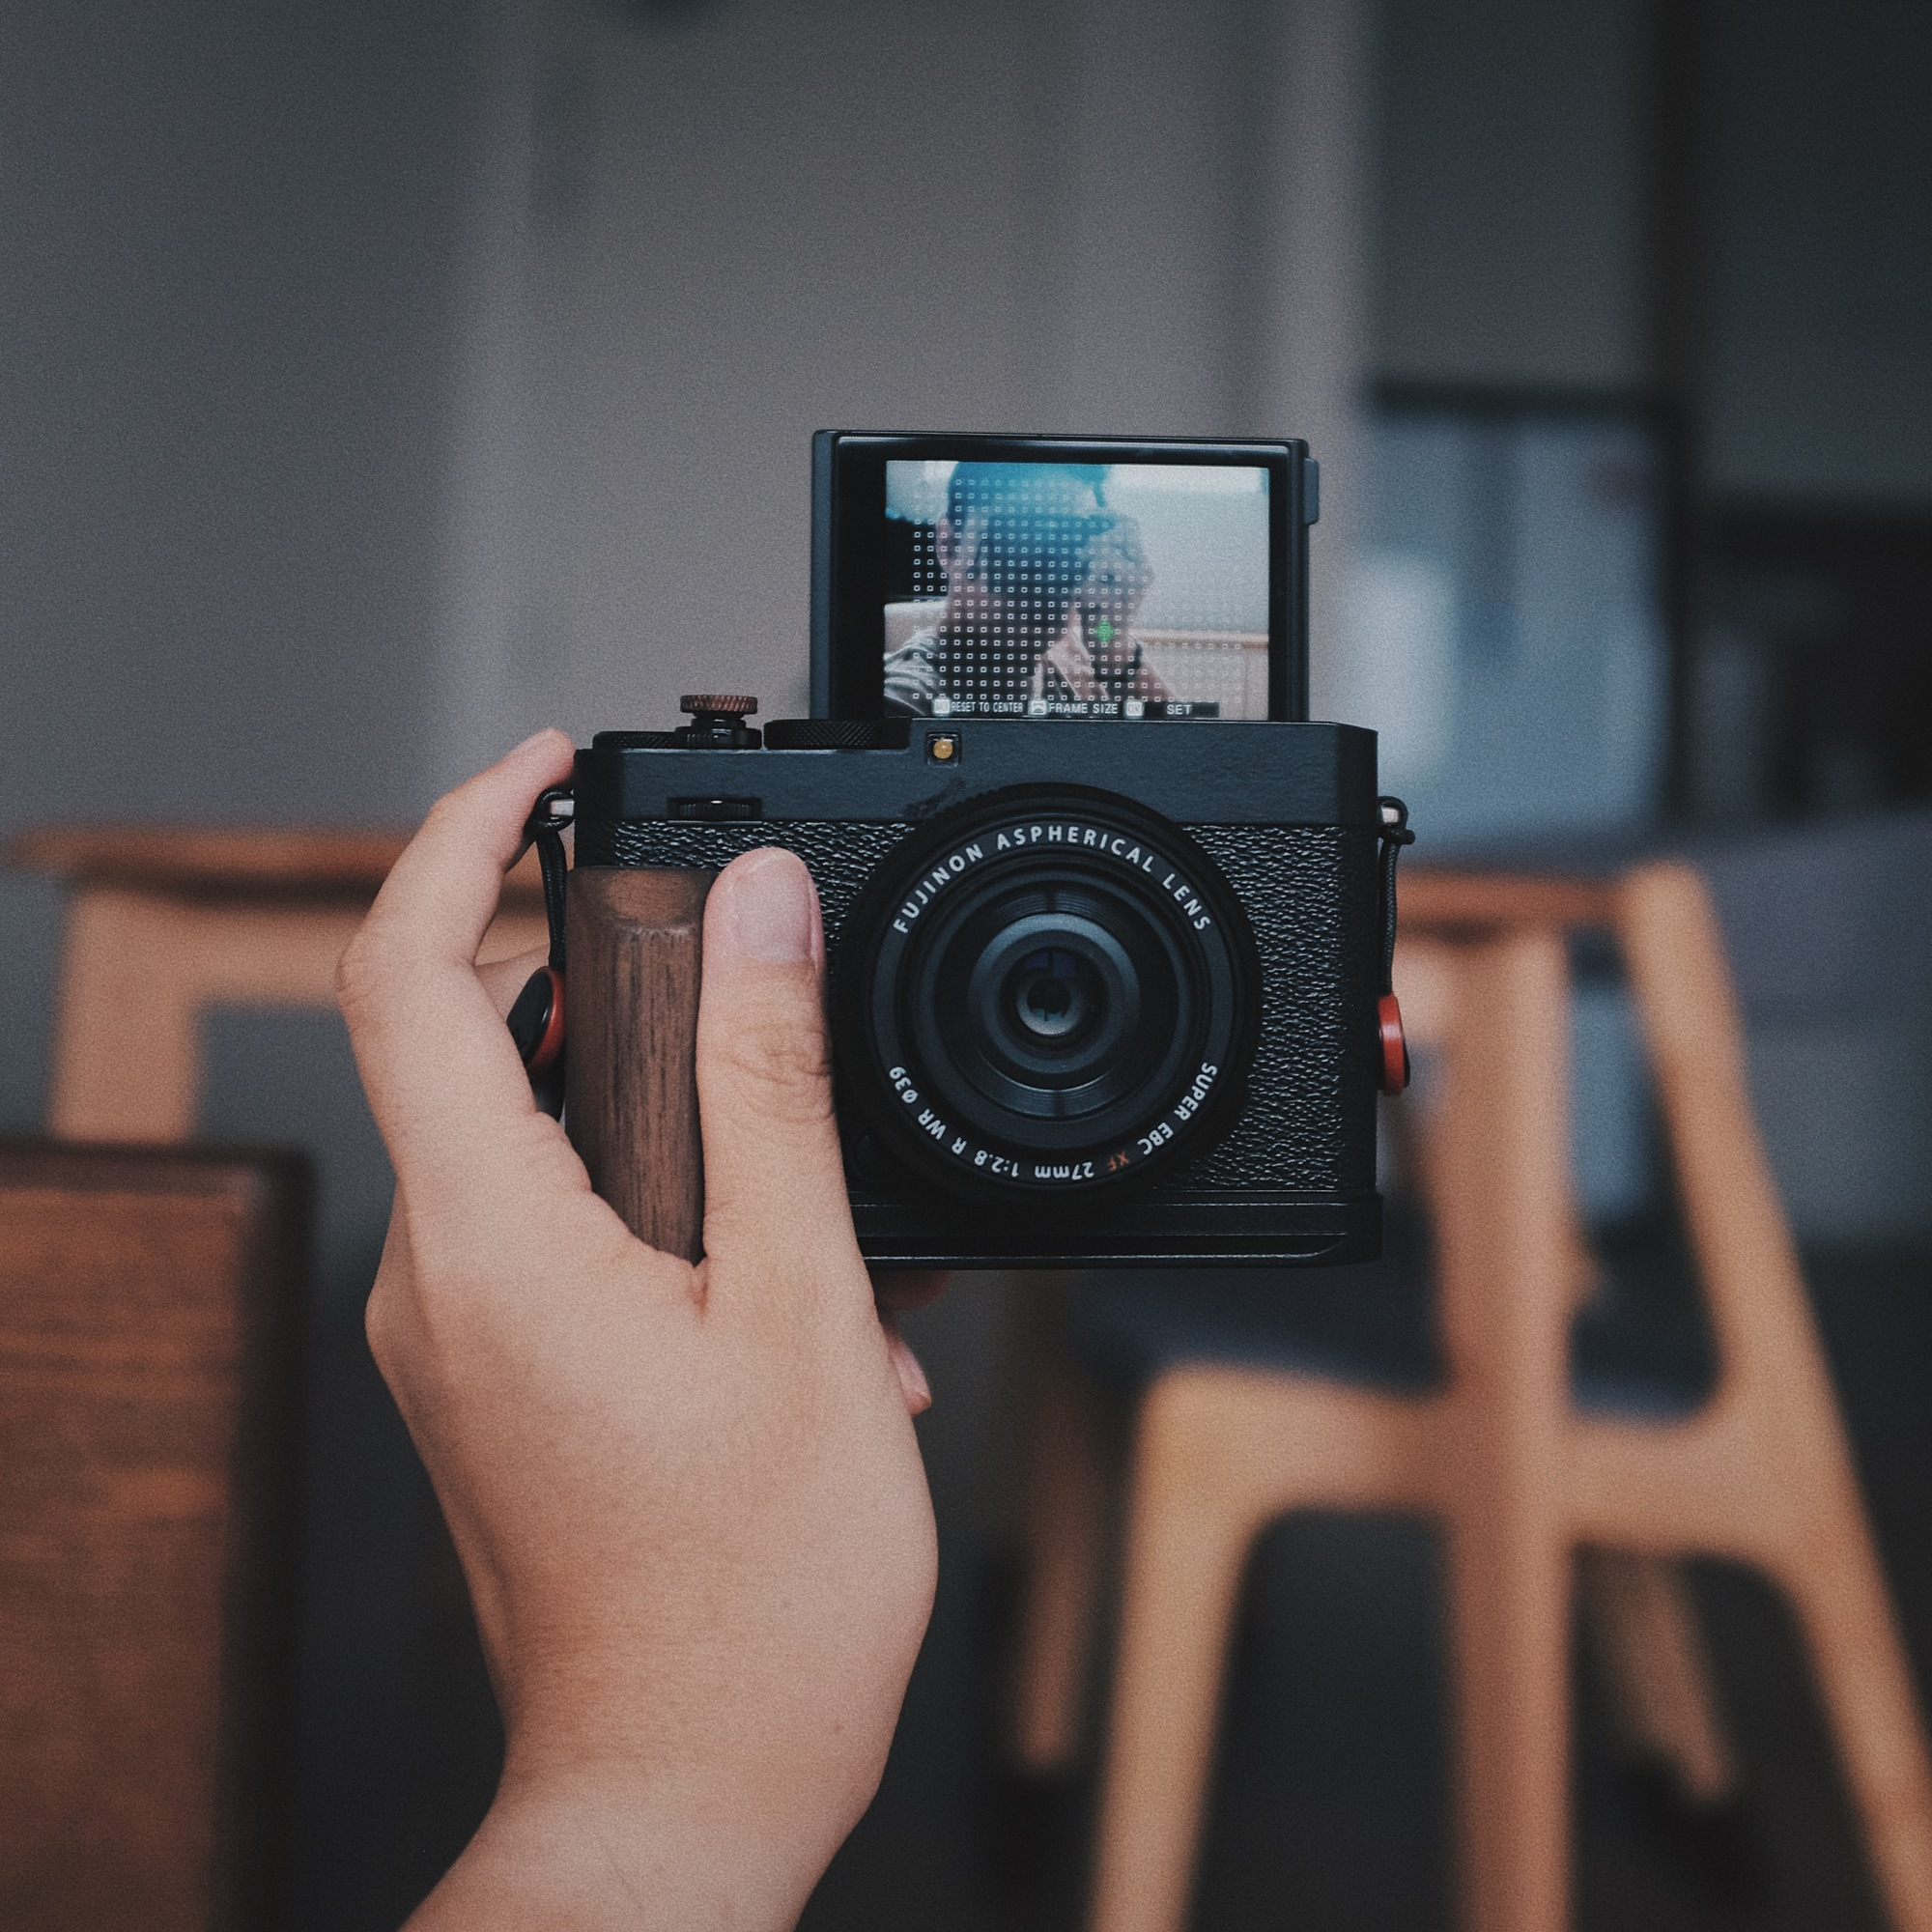
\includegraphics[width=\linewidth]{\envfinaldir/coverpic-prod.jpg}\par
            % \vskip 30pt
            \vfill

            \normalsize\rmfamily\scshape
            \copyright{} The Web Digest Project \hfill\large \envdatestr
        \end{center}
    \end{titlepage}
    % \restoregeometry
}
\newcommand{\simplehref}[1]{%
    \textcolor{blue!80!green}{\href{#1}{#1}}%
}
\renewcommand{\contentsname}{\center\Huge\sffamily\bfseries Contents\par\vskip 20pt}
\newcounter{ipartcounter}
\setcounter{ipartcounter}{0}
\newcommand{\ipart}[1]{
    % \vskip 20pt
    \clearpage
    \stepcounter{ipartcounter}
    \phantomsection
    \addcontentsline{toc}{chapter}{#1}
    % \begin{center}
    %     \Huge
    %     \sffamily\bfseries
    %     #1
    % \end{center}
    % \vskip 20pt plus 7pt
}
\newcounter{ichaptercounter}
\setcounter{ichaptercounter}{0}
\newcommand{\ichapter}[1]{
    % \vskip 20pt
    \clearpage
    \stepcounter{ichaptercounter}
    \phantomsection
    \addcontentsline{toc}{section}{\numberline{\arabic{ichaptercounter}}#1}
    \begin{center}
        \Huge
        \sffamily\bfseries
        #1
    \end{center}
    \vskip 20pt plus 7pt
}
\newcommand{\entrytitlefont}[1]{\subsection*{\raggedright\Large\sffamily\bfseries#1}}
\newcommand{\entryitemGeneric}[2]{
    % argv: title, url
    \parbox{\linewidth}{
        \entrytitlefont{#1}\par\vskip 5pt
        \footnotesize\ttfamily\mdseries
        \simplehref{#2}
    }\vskip 11pt plus 11pt minus 1pt
}
\newcommand{\entryitemGithub}[3]{
    % argv: title, url, desc
    \parbox{\linewidth}{
        \entrytitlefont{#1}\par\vskip 5pt
        \footnotesize\ttfamily\mdseries
        \simplehref{#2}\par\vskip 5pt
        \small\rmfamily\mdseries#3
    }\vskip 11pt plus 11pt minus 1pt
}
\newcommand{\entryitemAp}[3]{
    % argv: title, url, desc
    \parbox{\linewidth}{
        \entrytitlefont{#1}\par\vskip 5pt
        \footnotesize\ttfamily\mdseries
        \simplehref{#2}\par\vskip 5pt
        \small\rmfamily\mdseries#3
    }\vskip 11pt plus 11pt minus 1pt
}
\newcommand{\entryitemHackernews}[3]{
    % argv: title, hnurl, rawurl
    % \parbox{\linewidth}{
    %     \entrytitlefont{#1}\par\vskip 5pt
    %     \footnotesize\ttfamily\mdseries
    %     \simplehref{#3}\par
    %     \textcolor{black!50}{\href{#2}{#2}}
    % }\vskip 11pt plus 11pt minus 1pt
    \begin{minipage}{\linewidth}
            \entrytitlefont{#1}\par\vskip 5pt
            \footnotesize\ttfamily\mdseries
            \simplehref{#3}\par
            \textcolor{black!50}{\href{#2}{#2}}
    \end{minipage}\par\vskip 11pt plus 11pt minus 1pt
}







\begin{document}

\makeheader

\tableofcontents\clearpage




\ipart{Developers}
\ichapter{Hacker News}
\entryitemTwoLinks{Macrodata Refinement}{https://news.ycombinator.com/item?id=42902691}{https://lumon-industries.com/}

\entryitemTwoLinks{Phyllis Fong, who was investigating Neuralink, "forcefully removed "}{https://news.ycombinator.com/item?id=42902355}{https://timesofindia.indiatimes.com/technology/tech-news/phyllis-fong-who-was-investigating-elon-musks-brain-implant-startup-neuralink-forcefully-removed-from-office-after-refusing-termination-order/articleshow/117800543.cms}

\entryitemTwoLinks{Oracle Cloud deleting active user accounts without possibility for data recovery}{https://news.ycombinator.com/item?id=42901897}{https://mastodon.de/@ErikUden/113930010311998246}

\entryitemTwoLinks{Dell ends hybrid work policy, demands RTO despite remote work pledge}{https://news.ycombinator.com/item?id=42899975}{https://www.theregister.com/2025/01/31/dell\_ends\_hybrid\_work\_policy/}

\entryitemTwoLinks{ADHD Didn't Break Me–My Parents Did}{https://news.ycombinator.com/item?id=42899841}{https://claimingattention.substack.com/p/adhd-did-not-break-me-my-parents-did}

\entryitemTwoLinks{Bzip3: A spiritual successor to BZip2}{https://news.ycombinator.com/item?id=42899713}{https://github.com/kspalaiologos/bzip3}

\entryitemTwoLinks{Apple is open sourcing Swift Build}{https://news.ycombinator.com/item?id=42899703}{https://www.swift.org/blog/the-next-chapter-in-swift-build-technologies/}

\entryitemTwoLinks{Over 90\% of U.S. airport towers are understaffed, data shows}{https://news.ycombinator.com/item?id=42899261}{https://www.cbsnews.com/news/over-90-percent-u-s-airport-towers-understaffed-air-traffic-controllers-data-shows/}

\entryitemTwoLinks{The Zizians and the rationalist death cult}{https://news.ycombinator.com/item?id=42897871}{https://maxread.substack.com/p/the-zizians-and-the-rationalist-death}

\entryitemTwoLinks{CDC data are disappearing}{https://news.ycombinator.com/item?id=42897696}{https://www.theatlantic.com/health/archive/2025/01/cdc-dei-scientific-data/681531/}

\entryitemTwoLinks{FOSDEM 2025: Streaming Schedule}{https://news.ycombinator.com/item?id=42897254}{https://fosdem.org/2025/schedule/streaming/}

\entryitemTwoLinks{How to Run DeepSeek R1 671B Locally on a \$2000 EPYC Server}{https://news.ycombinator.com/item?id=42897205}{https://digitalspaceport.com/how-to-run-deepseek-r1-671b-fully-locally-on-2000-epyc-rig/}

\entryitemTwoLinks{Visualizing all books of the world in ISBN-Space}{https://news.ycombinator.com/item?id=42897120}{https://phiresky.github.io/blog/2025/visualizing-all-books-in-isbn-space/}

\entryitemTwoLinks{How to turn off Apple Intelligence}{https://news.ycombinator.com/item?id=42897041}{https://www.asurion.com/connect/tech-tips/turn-off-apple-intelligence/}

\entryitemTwoLinks{List of 200 UK companies that moved to 4-day working week}{https://news.ycombinator.com/item?id=42896387}{https://future4days.com/list-of-200-uk-companies-that-moved-to-4-day-working-week/}

\entryitemTwoLinks{Hell is overconfident developers writing encryption code}{https://news.ycombinator.com/item?id=42895332}{https://soatok.blog/2025/01/31/hell-is-overconfident-developers-writing-encryption-code/}

\entryitemTwoLinks{The government information crisis is bigger than you think it is}{https://news.ycombinator.com/item?id=42895331}{https://freegovinfo.info/node/14747/}

\entryitemTwoLinks{Hoppscotch: Open source alternative to Postman / Insomnia}{https://news.ycombinator.com/item?id=42895108}{https://github.com/hoppscotch/hoppscotch}

\entryitemTwoLinks{Decision to dump water from Tulare County lakes altered after confusing locals}{https://news.ycombinator.com/item?id=42894708}{https://sjvwater.org/decision-to-dump-water-from-tulare-county-lakes-altered-after-sending-locals-in-mad-scramble/}

\entryitemTwoLinks{All CDC data is no longer visible to comply with executive orders}{https://news.ycombinator.com/item?id=42894357}{https://www.cdc.gov/datainfo.html}\ichapter{Phoronix}
\entryitemGeneric{\hskip 0pt{}GTK's X11 Backend Now Deprecated, Planned For Removal In GTK 5}{https://www.phoronix.com/news/GTK-X11-Now-Deprecated}

\entryitemGeneric{\hskip 0pt{}gendwarfksyms Tool Added To Linux 6.14 To Help With Rust Push}{https://www.phoronix.com/news/Linux-6.14-gendwarfksyms}

\entryitemGeneric{\hskip 0pt{}Intel Battlemage, NVIDIA RTX 50 \& Linux Kernel Excitement From January}{https://www.phoronix.com/news/January-2025-Highlights}

\entryitemGeneric{\hskip 0pt{}Linux 6.14 RISC-V Kernel Adds Support For T-Head Vector Extensions, GhostWrite}{https://www.phoronix.com/news/Linux-6.14-RISC-V}

\entryitemGeneric{\hskip 0pt{}KDE Plasma 6.3: "It's Looking Pretty Good!"}{https://www.phoronix.com/news/KDE-Plasma-6.3-Looking-Good}

\entryitemGeneric{\hskip 0pt{}Wine Wayland Merge Request Opened For Clipboard Support}{https://www.phoronix.com/news/Wine-Wayland-Clipboard-Support}

\entryitemGeneric{\hskip 0pt{}"NOVA-Core" Patches Propose Building New NVIDIA Driver Piece-By-Piece In The Linux Kernel}{https://www.phoronix.com/news/NOVA-Core-Patches}

\entryitemGeneric{\hskip 0pt{}TLB Flushing Scalability Optimizations Merged For Linux 6.14 To Benefit AMD / Intel CPUs}{https://www.phoronix.com/news/Linux-6.14-TLB-Flush-Scalable}

\entryitemGeneric{\hskip 0pt{}GNOME 48 Switches Over To "Adwaita Sans" As Default Font}{https://www.phoronix.com/news/GNOME-48-Adwaita-Sans}\ichapter{Dribbble}
\entryitemGeneric{\hskip 0pt{}Atlantic Pickleball Club}{https://dribbble.com/shots/25558009-Atlantic-Pickleball-Club}

\entryitemGeneric{\hskip 0pt{}Stellar}{https://dribbble.com/shots/25559656-Stellar}

\entryitemGeneric{\hskip 0pt{}Wizard Logo}{https://dribbble.com/shots/25559490-Wizard-Logo}

\entryitemGeneric{\hskip 0pt{}Shuttle Robotics}{https://dribbble.com/shots/25557675-Shuttle-Robotics}

\entryitemGeneric{\hskip 0pt{}Real Estate Web Design}{https://dribbble.com/shots/25551949-Real-Estate-Web-Design}

\entryitemGeneric{\hskip 0pt{}Puzzle Fintech Website Design}{https://dribbble.com/shots/25501121-Puzzle-Fintech-Website-Design}

\entryitemGeneric{\hskip 0pt{}Columbus Bound®}{https://dribbble.com/shots/25550878-Columbus-Bound}

\entryitemGeneric{\hskip 0pt{}Vista Brand Identity}{https://dribbble.com/shots/25402719-Vista-Brand-Identity}

\entryitemGeneric{\hskip 0pt{}Team Heyo}{https://dribbble.com/shots/25539716-Team-Heyo}

\entryitemGeneric{\hskip 0pt{}Top of the World™ Hunt Club}{https://dribbble.com/shots/25545423-Top-of-the-World-Hunt-Club}

\entryitemGeneric{\hskip 0pt{}DeepSeek logo redesign}{https://dribbble.com/shots/25543483-DeepSeek-logo-redesign}

\entryitemGeneric{\hskip 0pt{}Abstro 8}{https://dribbble.com/shots/25546566-Abstro-8}

\entryitemGeneric{\hskip 0pt{}HappyDev - Logo Design (sold)}{https://dribbble.com/shots/25544140-HappyDev-Logo-Design-sold}

\entryitemGeneric{\hskip 0pt{}Illustration set}{https://dribbble.com/shots/25540370-Illustration-set}

\entryitemGeneric{\hskip 0pt{}VCC Unused Logo Concept - V6}{https://dribbble.com/shots/25543565-VCC-Unused-Logo-Concept-V6}

\entryitemGeneric{\hskip 0pt{}Year of the Snake}{https://dribbble.com/shots/25527312-Year-of-the-Snake}

\entryitemGeneric{\hskip 0pt{}Apparel}{https://dribbble.com/shots/25538973-Apparel}

\entryitemGeneric{\hskip 0pt{}2024 Logo Design Recap Pt.1}{https://dribbble.com/shots/25534698-2024-Logo-Design-Recap-Pt-1}

\entryitemGeneric{\hskip 0pt{}B}{https://dribbble.com/shots/25536900-B}

\entryitemGeneric{\hskip 0pt{}De Nieuwe Gemeente - Church Brand}{https://dribbble.com/shots/25537128-De-Nieuwe-Gemeente-Church-Brand}

\entryitemGeneric{\hskip 0pt{}Speed Test App Ui Design}{https://dribbble.com/shots/25535763-Speed-Test-App-Ui-Design}

\entryitemGeneric{\hskip 0pt{}Vintage Inspired}{https://dribbble.com/shots/25538473-Vintage-Inspired}

\entryitemGeneric{\hskip 0pt{}Plexo mobile app}{https://dribbble.com/shots/25534405-Plexo-mobile-app}

\entryitemGeneric{\hskip 0pt{}VCC Unused Logo Concept V5}{https://dribbble.com/shots/25534846-VCC-Unused-Logo-Concept-V5}


\ipart{Developers~~~~(zh-Hans)}
\ichapter{Solidot}
\entryitemGeneric{\hskip 0pt{}OpenAI 考虑开源旧模型}{https://www.solidot.org/story?sid=80459}

\entryitemGeneric{\hskip 0pt{}Bennu 小行星样本发现构成生命的基本成分}{https://www.solidot.org/story?sid=80458}

\entryitemGeneric{\hskip 0pt{}WhatsApp 称记者等成为以色列间谍软件的目标}{https://www.solidot.org/story?sid=80457}

\entryitemGeneric{\hskip 0pt{}朱诺号在木卫一上记录到至今最强的火山活动}{https://www.solidot.org/story?sid=80455}

\entryitemGeneric{\hskip 0pt{}新发现小行星有 1/83 的概率在 2032 年撞击地球}{https://www.solidot.org/story?sid=80454}

\entryitemGeneric{\hskip 0pt{}库克告诉张忠谋英特尔不知道如何代工芯片}{https://www.solidot.org/story?sid=80453}

\entryitemGeneric{\hskip 0pt{}巴塞尔税务机关因域名错误不得不购买巴哈马域名}{https://www.solidot.org/story?sid=80452}

\entryitemGeneric{\hskip 0pt{}美国版权局称 AI 辅助作品如果包含足够的人类创意可获得版权保护}{https://www.solidot.org/story?sid=80451}

\entryitemGeneric{\hskip 0pt{}LibreOffice 下载量突破 4 亿}{https://www.solidot.org/story?sid=80450}

\entryitemGeneric{\hskip 0pt{}Debian 项目停止在 X 上发推}{https://www.solidot.org/story?sid=80449}

\entryitemGeneric{\hskip 0pt{}Douglas Engelbart 诞辰 100 周年}{https://www.solidot.org/story?sid=80448}\ichapter{V2EX}
\entryitemGeneric{\hskip 0pt{}[互联网] upic 的错误日志该如何查看?在哪里查看}{https://www.v2ex.com/t/1108572}

\entryitemGeneric{\hskip 0pt{}[酷工作] 招全职 UIUX 设计师 | 类似闲鱼的社区属性二手票 APP,努力+氛围友好的纽约团队!(欢迎推荐, 8000 元奖励)}{https://www.v2ex.com/t/1108568}

\entryitemGeneric{\hskip 0pt{}[问与答] 有没有什么图片管理软件,可以自动对图片进行 OCR}{https://www.v2ex.com/t/1108567}

\entryitemGeneric{\hskip 0pt{}[分享创造] 小工具分享: DIY 谷歌服务令牌生成器(Photos \& Drive)}{https://www.v2ex.com/t/1108566}

\entryitemGeneric{\hskip 0pt{}[问与答] 如何劫持爸妈的网络,给他们推送点正常的东西}{https://www.v2ex.com/t/1108565}

\entryitemGeneric{\hskip 0pt{}[Docker] 感觉 Harbor 好难用}{https://www.v2ex.com/t/1108564}

\entryitemGeneric{\hskip 0pt{}[酷工作] 招游戏 2D 动画,插画师,接受远程全职/兼职}{https://www.v2ex.com/t/1108563}

\entryitemGeneric{\hskip 0pt{}[分享发现] [产品自荐] Celebrity Look Alike,一款使用 AI 技术帮你找到最像你的明星!}{https://www.v2ex.com/t/1108562}

\entryitemGeneric{\hskip 0pt{}[生活] 老婆想创业卖卤货,大家有什么建议吗?}{https://www.v2ex.com/t/1108561}

\entryitemGeneric{\hskip 0pt{}[程序员] 各位大佬,哪家机器搭建节点做亚马逊合适?}{https://www.v2ex.com/t/1108560}

\entryitemGeneric{\hskip 0pt{}[程序员] 如何进行大模型知识蒸馏}{https://www.v2ex.com/t/1108559}

\entryitemGeneric{\hskip 0pt{}[职场话题] deepseek 官网的接口挂了,推荐用第三方 SiliconCloud}{https://www.v2ex.com/t/1108558}

\entryitemGeneric{\hskip 0pt{}[分享发现] Windows 支持 sudo 了}{https://www.v2ex.com/t/1108557}

\entryitemGeneric{\hskip 0pt{}[Synology] 能通过 quick connect 连 webdav 么?}{https://www.v2ex.com/t/1108556}

\entryitemGeneric{\hskip 0pt{}[问与答] 问几个微信转 WeChat 的问题,求解答}{https://www.v2ex.com/t/1108555}

\entryitemGeneric{\hskip 0pt{}[问与答] 想携号转网到移动找个低价保号套餐求推荐}{https://www.v2ex.com/t/1108554}

\entryitemGeneric{\hskip 0pt{}[程序员] 用 deepseek r1 一天时间整了个终端 gpt 整合工具,方便阅读代码}{https://www.v2ex.com/t/1108552}

\entryitemGeneric{\hskip 0pt{}[问与答] 求馒头(m-team)的邀请}{https://www.v2ex.com/t/1108550}

\entryitemGeneric{\hskip 0pt{}[分享创造] 「新年送码」用 REFRAME 给照片加个蛇年水印 - 春节更新上线!}{https://www.v2ex.com/t/1108547}

\entryitemGeneric{\hskip 0pt{}[求职] c++多年经验求职}{https://www.v2ex.com/t/1108546}

\entryitemGeneric{\hskip 0pt{}[程序员] 为什么 LLM 模型不能按语言拆分,英文问题就只用英文语料训练出来的模型、日文问题就只用日文语料训练出来的模型,这样不是可以大幅减少参数量?}{https://www.v2ex.com/t/1108545}

\entryitemGeneric{\hskip 0pt{}[问与答] immich app 怎么上传单张照片,只发现备份功能}{https://www.v2ex.com/t/1108543}

\entryitemGeneric{\hskip 0pt{}[宽带症候群] 光猫是否有可能实现虚拟化?}{https://www.v2ex.com/t/1108542}

\entryitemGeneric{\hskip 0pt{}[职场话题] 年过完了,但是害怕找工作.}{https://www.v2ex.com/t/1108541}

\entryitemGeneric{\hskip 0pt{}[剧集] 大家似乎对剧版史密斯夫妇评价一般}{https://www.v2ex.com/t/1108540}

\entryitemGeneric{\hskip 0pt{}[信息安全] 来自 ipv6 only 的神秘问题,收到无法解析地址的流量}{https://www.v2ex.com/t/1108539}

\entryitemGeneric{\hskip 0pt{}[OpenWrt] 请教一个 openwrt + ipv6 + cloudflare 路由器回家的问题}{https://www.v2ex.com/t/1108536}

\entryitemGeneric{\hskip 0pt{}[Apple] 在 Safari 撤销文本输入是否有快捷键?}{https://www.v2ex.com/t/1108534}

\entryitemGeneric{\hskip 0pt{}[推广] Google 港区账号}{https://www.v2ex.com/t/1108533}

\entryitemGeneric{\hskip 0pt{}[生活] 父母过几年就能退休拿养老金,工作不辛苦,平时打打牌跳跳舞,日子可以过得很好,却一定要在工作和个人问题上激化矛盾,既然无法沟通不如不回家}{https://www.v2ex.com/t/1108532}

\entryitemGeneric{\hskip 0pt{}[问与答] 离过婚 比 没结婚 强吗?}{https://www.v2ex.com/t/1108531}

\entryitemGeneric{\hskip 0pt{}[分享发现] 硅基流动第 1 天支持 DeepSeek V3 和 R1, 还算是稳定}{https://www.v2ex.com/t/1108530}

\entryitemGeneric{\hskip 0pt{}[问与答] 求各位佬推荐一些好玩的项目}{https://www.v2ex.com/t/1108528}

\entryitemGeneric{\hskip 0pt{}[问与答] 笔记本的触控板那总容易进灰,请问各位是如何解决的}{https://www.v2ex.com/t/1108527}

\entryitemGeneric{\hskip 0pt{}[Vue.js] 请教 Vue3 + typescript 最佳实践问题}{https://www.v2ex.com/t/1108526}

\entryitemGeneric{\hskip 0pt{}[程序员] 免费开源 AI 简历编辑器-魔方简历, DeepSeek, 豆包大模型驱动}{https://www.v2ex.com/t/1108525}

\entryitemGeneric{\hskip 0pt{}[Python] [蛇年进阶 Python !] 过年蹲家里翻译了本书《Cosmic Python 》,楼主认为是 Python 届的 DDD(领域驱动设计)手把手喂饭教学}{https://www.v2ex.com/t/1108524}

\entryitemGeneric{\hskip 0pt{}[区块链] 汇丰蓝狮扣账卡绑定 apple pay 在币安 app 法币购买 BTC 失败}{https://www.v2ex.com/t/1108523}

\entryitemGeneric{\hskip 0pt{}[问与答] 电报群里都有啥好东西呢?}{https://www.v2ex.com/t/1108522}

\entryitemGeneric{\hskip 0pt{}[分享发现] MasterCard 官网活动数据库疑似被脱,请参加过去年 Master 港卡返现活动的及时锁卡报失}{https://www.v2ex.com/t/1108520}

\entryitemGeneric{\hskip 0pt{}[分享发现] DeepSeek 与主流 AI 模型对比评测}{https://www.v2ex.com/t/1108519}

\entryitemGeneric{\hskip 0pt{}[Apple] iPhone 16 Pro Apple Pay 无法重新添加部分卡片,求解方案}{https://www.v2ex.com/t/1108518}

\entryitemGeneric{\hskip 0pt{}[电影] 哪吒 2 要冲击中国影史票房?}{https://www.v2ex.com/t/1108516}

\entryitemGeneric{\hskip 0pt{}[问与答] 亲宝宝怎么批量下载图片视频}{https://www.v2ex.com/t/1108515}

\entryitemGeneric{\hskip 0pt{}[程序员] XXL-RPC v1.9.0 | RPC 服务框架}{https://www.v2ex.com/t/1108514}

\entryitemGeneric{\hskip 0pt{}[Telegram] 有没有朋友买过 TG 的成品号}{https://www.v2ex.com/t/1108513}

\entryitemGeneric{\hskip 0pt{}[NAS] 关于 TrueNas 的 core 和 scale(2025.1.28-1.31 使用体验)}{https://www.v2ex.com/t/1108512}

\entryitemGeneric{\hskip 0pt{}[汽车] 2025 年,求推荐 15w 以内的电车或油车,硬性指标:后备箱能装得下一个折叠轮椅}{https://www.v2ex.com/t/1108511}

\entryitemGeneric{\hskip 0pt{}[Chrome] 天塌了, chrome 的扩展大面积失效}{https://www.v2ex.com/t/1108510}

\entryitemGeneric{\hskip 0pt{}[生活] 春节回家发现农村人迷信赤脚医生}{https://www.v2ex.com/t/1108508}


\ipart{Generic News}







\clearpage
\leavevmode\vfill
\footnotesize

Copyright \copyright{} 2023-2025 Neruthes and other contributors.

This document is published with CC BY-NC-ND 4.0 license.

The entries listed in this newsletter may be copyrighted by their respective creators.

This newsletter is generated by the Web Digest project.

The newsletters are also delivered via Telegram channel \CJKunderline{\href{https://t.me/webdigestchannel}{https://t.me/webdigestchannel}}.\\
RSS feed is available at \CJKunderline{\href{https://webdigest.pages.dev/rss.xml}{https://webdigest.pages.dev/rss.xml}}.

This newsletter is available in PDF at
\CJKunderline{\href{https://webdigest.pages.dev/}{https://webdigest.pages.dev/}}.

The source code being used to generate this newsletter is available at\\
\CJKunderline{\href{https://github.com/neruthes/webdigest}{https://github.com/neruthes/webdigest}}.

This newsletter is also available in
\CJKunderline{\href{http://webdigest.pages.dev/readhtml/\envyear/WebDigest-20250202.html}{HTML}} and
\CJKunderline{\href{https://github.com/neruthes/webdigest/blob/master/markdown/\envyear/WebDigest-20250202.md}{Markdown}}.


\coverpic{https://unsplash.com/photos/a-view-of-a-mountain-range-with-a-church-in-the-foreground-STI61Ubba4Q}{Pascal Bullan}


\end{document}
